% -*- latex -*-
%%%%%%%%%%%%%%%%%%%%%%%%%%%%%%%%%%%%%%%%%%%%%%%%%%%%%%%%%%%%%%%%
%%%%%%%%%%%%%%%%%%%%%%%%%%%%%%%%%%%%%%%%%%%%%%%%%%%%%%%%%%%%%%%%
%%%%
%%%% This text file is part of the source of 
%%%% `Parallel Programming in MPI and OpenMP'
%%%% by Victor Eijkhout, copyright 2012-9
%%%%
%%%% mpi-running.tex : about running MPI programs
%%%%
%%%%%%%%%%%%%%%%%%%%%%%%%%%%%%%%%%%%%%%%%%%%%%%%%%%%%%%%%%%%%%%%
%%%%%%%%%%%%%%%%%%%%%%%%%%%%%%%%%%%%%%%%%%%%%%%%%%%%%%%%%%%%%%%%

\Level 0 {Starting and running MPI processes}
\label{sec:mpi-start}

The \ac{SPMD} model may be initially confusing. Even though there is
only a single source, compiled into a single executable,
the parallel run comprises a number of independently started MPI
processes (see section~\ref{sec:mpiexec} for the mechanism).

The following exercises are designed to give you an intuition for this
one-source-many-processes setup. In the first exercise you will see
that the mechanism for starting MPI programs starts up independent
copies. There is nothing in the source that says `and now you become parallel'.

\begin{figure}[ht]
  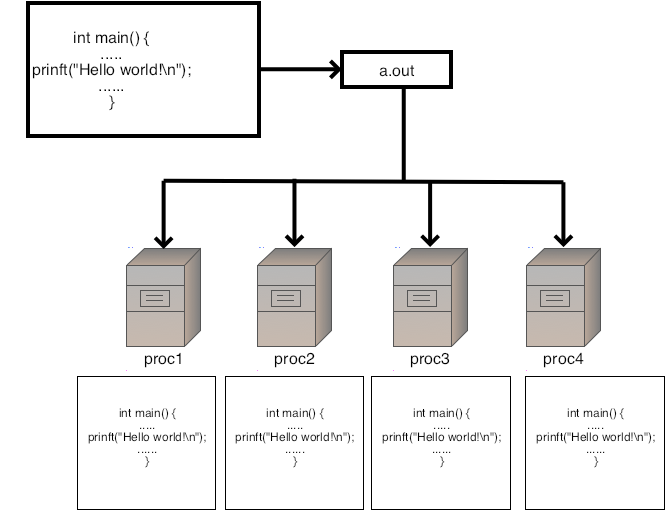
\includegraphics[scale=.5]{hello-parallel}
  \caption{Running a hello world program in parallel}
  \label{fig:hello-parallel}
\end{figure}

%pyinput ex.txt

The following exercise demonstrates this point.

\begin{exercise}
  \label{ex:hello1}
  Write a `hello world' program, without any MPI in it,
  and run it in parallel with \indextermtt{mpiexec} or your local equivalent. 
  Explain the output.

\begin{tacc}
    (On TACC machines such as stampede, use \indextermtt{ibrun}, no
    processor count.)
\end{tacc}

\end{exercise}

This exercise is illustrated in figure~\ref{fig:hello-parallel}.

\Level 1 {Headers}

If you use MPI commands in a program file, be sure to include
the proper header file, \indexterm{mpi.h} or \indexterm{mpif.h}.
\begin{verbatim}
#include "mpi.h" // for C
#include "mpif.h" ! for Fortran
\end{verbatim}
For \emph{Fortran90}\index{Fortran!Fortran90}, many MPI installations
also have an MPI module, so you can write
\begin{verbatim}
use mpi     ! pre 3.0
use mpi_f08 ! 3.0 standard
\end{verbatim}
The internals of these files can be different between MPI
installations, so you can not compile one file against one \n{mpi.h}
file and another file, even with the same compiler on the same machine,
against a different MPI.

\Level 1 {Initialization / finalization}
\label{sec:mpi-init}

To get a useful MPI program you need at least the calls
\indexmpishow{MPI_Init} and \indexmpishow{MPI_Finalize} surrounding
your code.

\begin{pythonnote}
  There are no initialize and finalize calls: the \n{import} statement
  performs the initialization.
\end{pythonnote}

Every MPI program has to start with \indextermbus{MPI}{initialization}:
%
\mpiRoutineRef{MPI_Init}
%
where \indextermtt{argc} and \indextermtt{argv} are the arguments
of a C language main program:
\lstset{style=reviewcode,language=C}
 \begin{lstlisting}
int main(int argc,char **argv) {
    ....
    return 0;
}
\end{lstlisting}
(It is allowed to pass \n{NULL} for these arguments.)

Note that the \indexmpishow{MPI_Init} call is one of the few that differs between C and Fortran:
the C~routine takes the commandline arguments, which Fortran lacks.

This may look a bit like declaring `this is the parallel part of a
program', but that's not true: again, the whole code is executed
multiple times in parallel.

The regular way to conclude an MPI program is:
%
\mpiRoutineRef{MPI_Finalize}

\begin{exercise}
  \label{ex:hello2}
  Add the commands \indexmpishow{MPI_Init} and \indexmpishow{MPI_Finalize}
  to your code. Put three different print statements in your code: one before the init,
  one between init and finalize, and one after the finalize. Again explain the output.
\end{exercise}

\Level 2 {Aborting an MPI run}

Apart from \indexmpishow{MPI_Finalize}, which signals a successful
conclusion of the MPI run, an abnormal end to a run can be forced by
\indexmpishow{MPI_Abort}:
%
\mpiRoutineRef{MPI_Abort}
%
This aborts execution on all processes associated with the communicator,
but many implementations simply abort all processes. The \n{value} parameter
is returned to the environment.

\Level 2 {Testing the initialized/finalized status}

The commandline arguments \n{argc} and \n{argv} are only guaranteed to
be passed to process zero, so the best way to pass commandline information
is by a broadcast (section~\ref{sec:bcast}).

There are a few commands, such as
\indexmpishow{MPI_Get_processor_name}, that are allowed before
\indexmpishow{MPI_Init}.

If MPI is used in a library, MPI can have already been initialized in a main program.
For this reason, one can test where \indexmpishow{MPI_Init} has been called with
%
\mpiRoutineRef{MPI_Initialized}
%

You can test whether \indexmpishow{MPI_Finalize} has been called with
%
\mpiRoutineRef{MPI_Finalized}

\Level 2 {Commandline arguments}

The \indexmpishow{MPI_Init} routines takes a reference to \indextermtt{argc}
and \indextermtt{argv} for the following reason: the \indexmpishow{MPI_Init} calls
filters out the arguments to \indexterm{mpirun} or \indexterm{mpiexec},
thereby lowering the value of \n{argc} and elimitating some of the \n{argv}
arguments.

On the other hand, the commandline arguments that are meant for \n{mpiexec}
wind up in the \indexmpishow{MPI_INFO_ENV} object as a set of
key/value pairs; see section~\ref{sec:mpi-info}

\Level 2 {Information about the run}

Once MPI has been initialized, the \indexmpishow{MPI_INFO_ENV} object
contains a number of key/value pairs describing run-specific
information; see section~\ref{sec:mpi-info-env}.
